% Figure s04f03_guidingcenter (Session 4): why the Landau levels are flat.
% The image is rendered by figures/blender/s04f03_guidingcenter.py; the coordinates of the labels come from
% figures/blender/out/s04f03_guidingcenter_anchors.tex. Build with figures/blender/build_figure.sh s04f03_guidingcenter.
\documentclass[11pt,tikz,border=0pt]{standalone}
\usepackage[T1]{fontenc}
\usepackage{amsmath,amssymb,graphicx,bm}
\usepackage{xcolor}
\usetikzlibrary{arrows.meta,calc}
% The three label colors of the figures, with the same values as in src/figures_preamble.tex.
\definecolor{aqmaccent}{RGB}{31,78,121}
\definecolor{aqmbroken}{RGB}{168,42,34}
\definecolor{aqmmuted}{RGB}{125,125,125}

\newlength{\figw}\setlength{\figw}{16.17cm}   % 1.04 of the text width, before the empty margins of the render are cropped

\begin{document}
\begin{tikzpicture}[lbl/.style={font=\small, inner sep=1.5pt}, pnl/.style={font=\small\bfseries, inner sep=1.5pt}]
  \node[overlay, anchor=south west, inner sep=0pt] at (0,0)
    {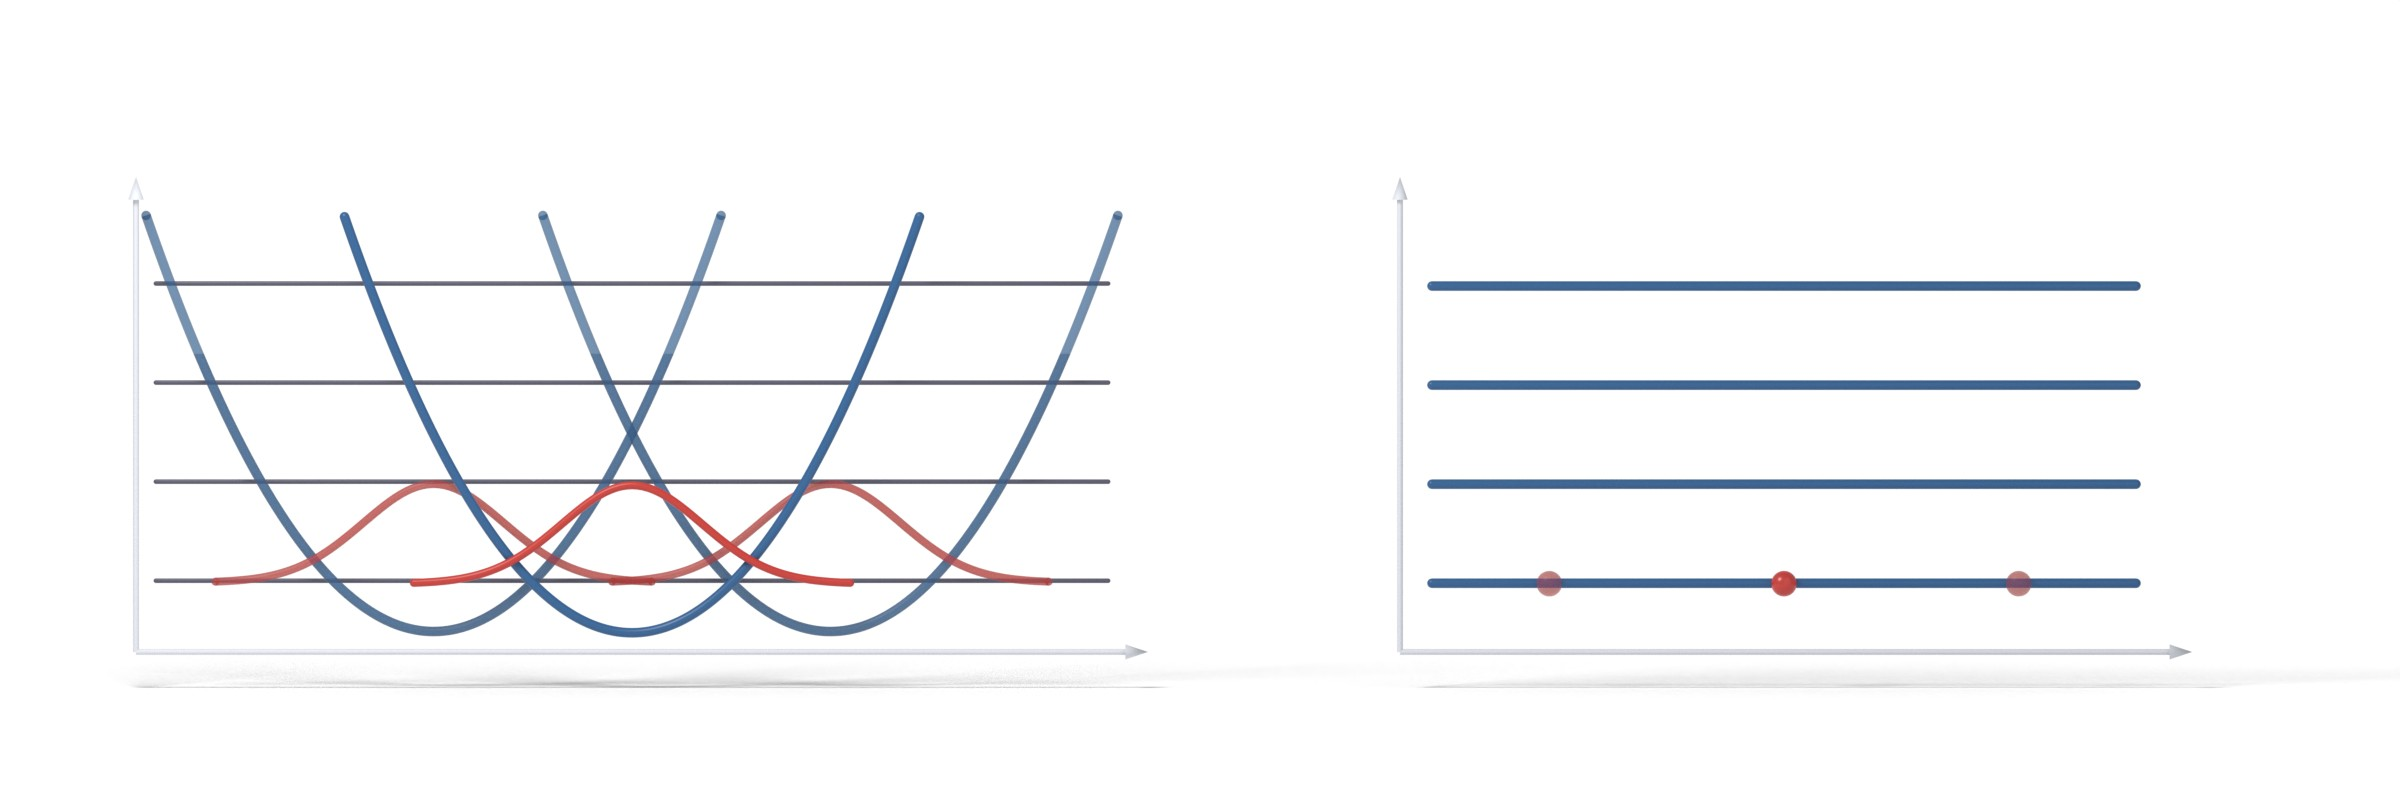
\includegraphics[width=\figw]{../blender/out/s04f03_guidingcenter.jpg}};
  % written by build_figure.sh; the painted part of the image
\path (0.0533\figw,0.0454\figw) rectangle (0.9958\figw,0.2596\figw);

  %% written by figlib.py; x and y in units of the image width
\coordinate (x0) at (0.1807\figw,0.0564\figw);
\coordinate (x1) at (0.2633\figw,0.0564\figw);
\coordinate (x2) at (0.3460\figw,0.0564\figw);
\coordinate (ax) at (0.4783\figw,0.0617\figw);
\coordinate (aE) at (0.0567\figw,0.2595\figw);
\coordinate (apanel) at (0.0500\figw,0.2760\figw);
\coordinate (E0) at (0.0567\figw,0.0903\figw);
\coordinate (E1) at (0.0567\figw,0.1316\figw);
\coordinate (E2) at (0.0567\figw,0.1729\figw);
\coordinate (E3) at (0.0567\figw,0.2141\figw);
\coordinate (k0) at (0.6456\figw,0.0564\figw);
\coordinate (k1) at (0.7433\figw,0.0564\figw);
\coordinate (k2) at (0.8411\figw,0.0564\figw);
\coordinate (bx) at (0.9133\figw,0.0617\figw);
\coordinate (bE) at (0.5833\figw,0.2595\figw);
\coordinate (bpanel) at (0.5767\figw,0.2760\figw);

  \node[pnl, anchor=south west] at (apanel) {(a)};
  \node[pnl, anchor=south west] at (bpanel) {(b)};
  \node[lbl, anchor=south east] at (ax) {$x$};
  \node[lbl, anchor=south east] at (bx) {$k_y$};
  \node[lbl, anchor=west] at (aE) {$E$};
  \node[lbl, anchor=west] at (bE) {$E$};
  \foreach \n/\t in {0/{\tfrac12},1/{\tfrac32},2/{\tfrac52},3/{\tfrac72}} { \node[lbl, anchor=east] at (E\n) {$\t$}; }
  \node[lbl, anchor=north] at ($(x1)+(0,-0.12cm)$) {guiding centres $x_0=\hbar k_y/B$};
\end{tikzpicture}
\end{document}
